\chapter{Sprint 1}

\minitoc

\subsubsection{Purpose}

This chapter will outline the work we did in the first sprint. It explains in detail how we planned the sprint, including which user stories we chose and the architecture we employed to implement these. Details on the implementation on each user story is also included, as well documentation on the testing process. Finally our evaluation of the first sprint is presented. 

\clearpage

\section{Planning}
We started the sprint with a sprint planning meeting September 24th. The plan for this sprint was to implement a basic implementation of the system, so that we would have something to show the customer at the end of the sprint. We chose user stories from the backlog that would enable us to this, a client and server offering only the most basic operations. 

\subsection{Duration}
This sprint started on September 24th and lasted for two weeks. A customer demo was held at October 4th to show of what we have achieved during the sprint and to ensure that the customer agreed with the implementation.

\subsection{Sprint Goal}
The goal for the first sprint was to get a basic version of the library application working. This included creating a basic GUI with both the graphical web- application and the console side by side, creating a server capable of storing objects and establish communication between the server and client through a basic REST api. The user should be able to use both the web- application and the console to add a new book to the system and to list the books currently in the system. In addition we decided to implement the real- time messaging from the server to the clients to verify that the solution we chose in the pre- study would be up to the task.

\subsection{Product Backlog}
For the first sprint, we used the user stories from the initial requirements as our product backlog. The full product backlog for Sprint 1 can be found in section \ref{sprint1pb} in the appendix.

\subsection{Sprint Backlog}
The user stories we chose to include in the sprint backlog with their estimated workload is listed in Table~\ref{table:sp1backlog}. We estimated that we have around 160 hours each sprint for working with the actual user stories. The remaining 40 hours would be used for meetings, demonstrations and project management.

Following is some points to discuss the deviations in estimated effort and actual time used.
\begin{itemize}
\item We used more time on implementation than we planned for. We are still getting used to the fact that we have to document everything, usually we only expend effort towards the actual coding process. Also we had to spend some time setting up technologies on a server and get them running before we started implementing actual functionality.
\item We used less time on design than we planned. Still getting used to designing everything before we code, up front. We plan to do this better the next sprint
\item We used quite a lot of time less on testing than we estimated. We anticipated that we had to use a considerable time to correct bugs and errors during the testing, but all the test cases passed on the first attempt. We anticipated that we had to spend more time on getting all the technologies we had chosen to play together nicely through extensive testing, but it turned out that they were a great fit, and that it wasn't too much work to get them working together in the way we intended.
\item Once we had implemented the functionality of adding new books, the time used to implement D2 and D5 was considerably reduced, as we could resuse much of the code we had created for D1.
\item The PubNub real- time messaging turned out to be easier to implement with Node.js than we expected. 
\item We ended up spending more time on the Scrum planning meeting than we planned for. In addition we didn't work as many hours that we planned for. As a result we had less time available to implement the user stories. Luckily the it turned out that this time was sufficient to finish all the user stories we planned to implement.
\end{itemize}

\begin{table}
\caption{Sprint 1 Backlog}
\centering
\begin{tabular}{ l p{8cm} l l }
\hline 
			&				&\multicolumn{2}{c}{Hours}			\\
 User Story	& Short Description		&Est.		&Act.	                               \\ 
\hline \\ [-2.0ex]
 \bf{A1}     &\bf{Store objects in database}		&\bf{30}		&\bf{40}          \\ 
		  &Design							&8			&6		\\
		  &Implementation					&15			&25		\\
		  &Testing						&4			&4		\\
		  &Documentation					&3			&5		\\

 \bf{A2}     &\bf{Send real- time messages} 		&\bf{20}		&\bf{13}               \\ 
		  &Design							&4			&2		\\
		  &Implementation					&10			&7		\\
		  &Testing						&4			&3		\\
		  &Documentation					&2			&1		\\

 \bf{A3}     &\bf{Access to domain specific object} 	&\bf{25}		&\bf{22}		     \\ 
		  &Design							&10			&5		\\
		  &Implementation					&10			&10		\\
		  &Testing						&3			&3		\\
		  &Documentation					&2			&4		\\

 \bf{G3}     &\bf{Graphical web- application and console}		&\bf{35}		&\bf{38}		     \\ 
		  &Design							&12			&10		\\
		  &Implementation					&15			&21		\\
		  &Testing						&4			&2		\\
		  &Documentation					&4			&5		\\

 \bf{D1}	  &\bf{Add a new book}				&\bf{15}		&\bf{18}		     \\
		  &Design							&3			&2		\\
		  &Implementation					&8			&12		\\
		  &Testing						&2			&2		\\
		  &Documentation					&2			&2		\\

\bf{D2}	  &\bf{Delete a book}				&\bf{15}		&\bf{7}		     \\
		  &Design							&3			&1		\\
		  &Implementation					&8			&4		\\
		  &Testing						&2			&1		\\
		  &Documentation					&2			&1		\\

 \bf{D5}	  &\bf{List all the books in the system}	&\bf{20}		&\bf{9}		     \\
		  &Design							&5			&2		\\
		  &Implementation					&10			&5		\\
		  &Testing						&3			&1		\\
		  &Documentation					&2			&1		\\
\hline 
		  &\bf{Total:}						&\bf{160}		&\bf{147}		\\
\hline
\end{tabular}
\label{table:sp1backlog}
\end{table}

\begin{table}
\caption{Sprint 1 Workload}
\centering
\begin{tabular}{ l l l }
\hline 
			&\multicolumn{2}{c}{Hours}			\\
 Task		&Est.			&Act.	                               \\ 
\hline \\ [-2.0ex]
Design			&45		&28		\\
Implementation	&76		&84		\\
Testing			&22		&16		\\
Documentation	&17		&19		\\
\hline
\bf{Total}			&\bf{160}	&\bf{147}		\\
\hline
\end{tabular}
\label{table:sp1workload}
\end{table}


\section{Architecture}
This section will handle the architecture we used for this sprint. The architecture will be described through class diagram and component diagram.


\subsection{4+1 view model}
The 4+1 view model\cite{Kruchten}. Here the views will be described as they are in sprint 1, and how they will look in our architecture. 

\subsubsection{Logical View}
Describes the functionality in the system from the end users perspective.The end users will mainly be power users, wanting to perform object editing tasks efficiently. This view will be described through class, communication and sequence diagram.

\begin{figure}[h]
\centering
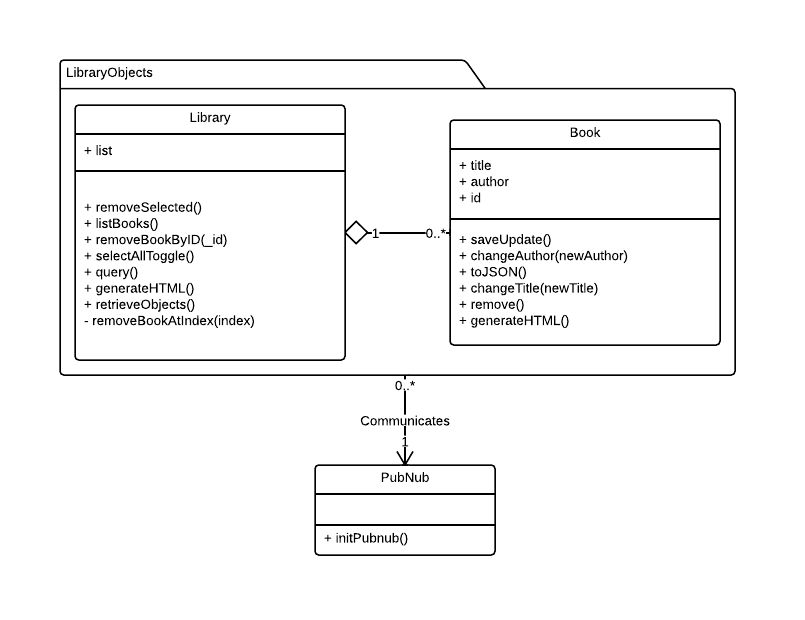
\includegraphics[width=6in]{image/architecture/s1/s1clientClassDiagram.png}
\caption{Client Class Diagram}
\label{figure:s1clientClassDiagram}
\end{figure}

Figure~\ref{figure:s1clientClassDiagram} The client class diagram gives an overview of the class structure of system, and how they collaborate. We can see that the client consists of two separate views, a GUI and a Shell, which is split by a splitpane so the user can se bouth a GUI interface and the commandline interface. These two views can make changes to the library objects, and get reflected back to the other view. The library objects consists of a library filed with books. The changes done to a book is delivered to other clients and the server through PubNub. 

\begin{figure}[h]
\centering
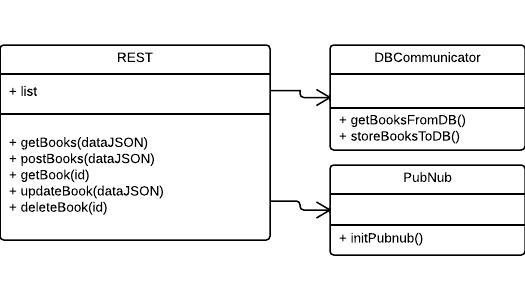
\includegraphics[width=5in]{image/architecture/s1/s1serverClassDiagram.png}
\caption{Client Class Diagram}
\label{figure:s1serverClassDiagram}
\end{figure}

Figure~\ref{figure:s1serverClassDiagram} The server class diagram shows how the REST api is set up, and the communication with the pubnub and db where the library information is stored.


%\subsubsection{Process View}
%Describes the dynamic aspect of the system, and explains how the different parts of the system will communicate at runtime. This is described with a activity diagram.

%The user will ask for an object from the backend, this will be delivered to the client through the communication channel as a json object, the client will interpret this and the user can then edit it through the console, and send it back to the backend.



\subsubsection{Physical View}
Describes the system from the system engineer's perspective. And explains the physical connections between the software components. Described through a deployment diagram. 

\begin{figure}[h]
\centering
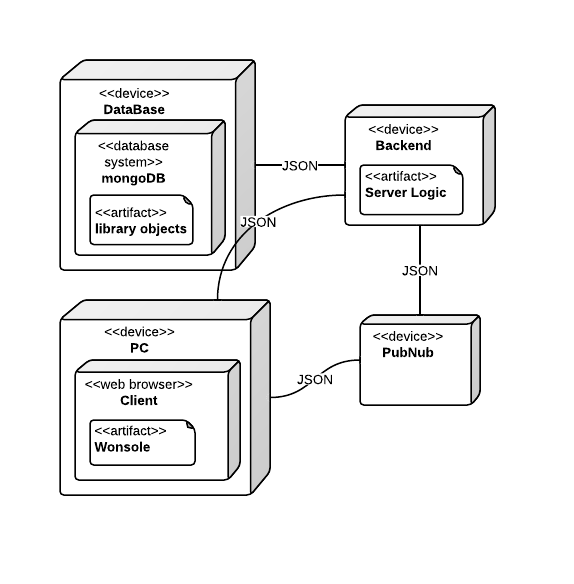
\includegraphics[width=5in]{image/architecture/s1/s1DeploymentDiagram.png}
\caption{Deployment Diagram}
\label{figure:s1DeploymentDiagram}
\end{figure}

Figure~\ref{figure:s1DeploymentDiagram} The structure of the four different parts of the system.

\subsubsection{Development View}
Describes the system from the programmer's perspective. This will be described through how the different component parts are separated. Component and package diagrams will show this.

\begin{figure}[h]
\centering
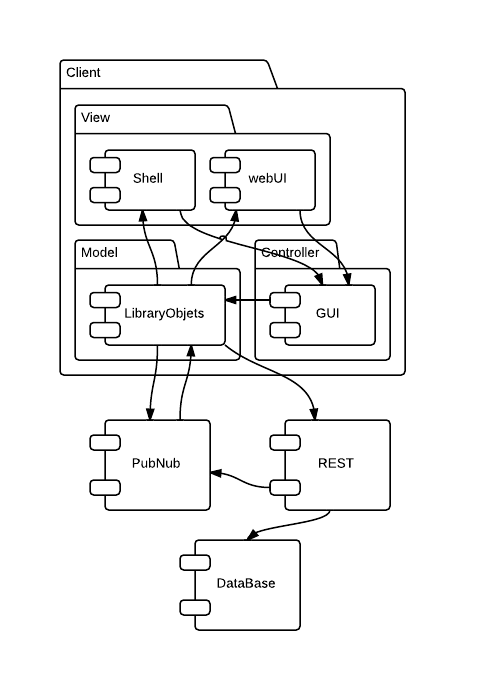
\includegraphics[width=5in]{image/architecture/s1/s1ComponentDiagram.png}
\caption{Component Diagram}
\label{figure:s1ComponentDiagram}
\end{figure}

Figure~\ref{figure:s1ComponentDiagram} These components form a three layered structure, and communicate with each other through the neighboring layer.


\section{Implementation}

\subsection{RESTful API}
We decided to expose the contents of the database on the central server to the clients through a RESTful API that is served over HTTP. REST is an abbreviation for REpresentational State Transfer, and it basically allows you to get information and perform action equipped only with URLs and standard HTTP methods like GET and POST. The point of REST is having one standard interface for any service. Instead of exposing an interface which has methods, you only expose 4 methods; create, update, read and delete.  You use the URL to describe what object you are performing the action on.

A detailed explanation of the RESTful is included in the appendices. In addition example code with jQuery(JavaScript) will be supplied.

\subsection{Client-side application}

See Figure~\ref{figure:Wonsole-Sprint1}.

\begin{figure}
\centering
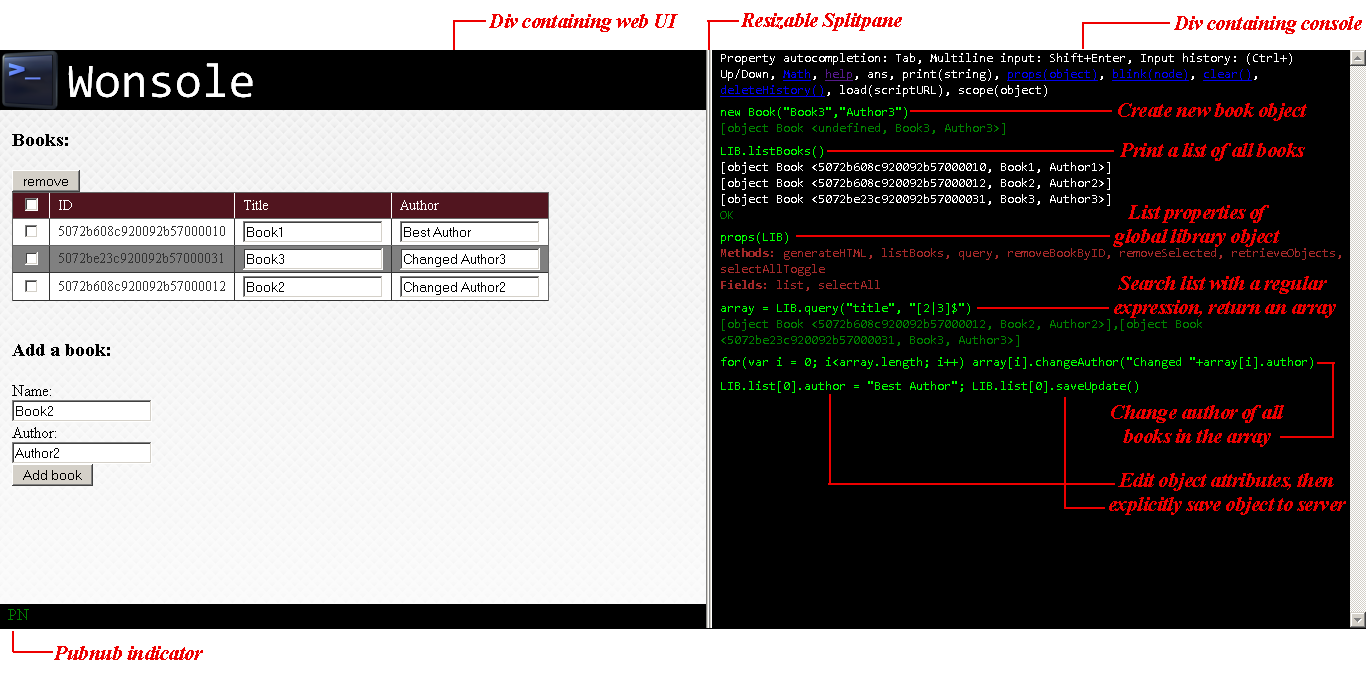
\includegraphics[width=6in]{image/Wonsole-Sprint1.png}
\caption{Wonsole, Sprint 1}
\label{figure:Wonsole-Sprint1}
\end{figure}

\subsubsection{Web UI}
The web user interface is a standard HTML/CSS web site. Lists of objects and their information are generated through JavaScript, and UI elements are associated with JavaScript methods to perform changes to the underlying objects.

\subsubsection{JavaScript Console}
For the console part of the UI, we decided to build off of an existing implementation. We used JavaScript Shell 1.4, which is a command-line interface for JavaScript and DOM. The console will be rather heavily modified to suit the needs of our project. The console current supports a number of useful features, such as listing the variables and methods of an object, suggestions, and a command history. In later sprints, we intend to implement more useful autocompletion, easier navigation of lists of objects as well as better visualization of objects and better integration with the web UI.

The JavaScript Shell is GPL/LGPL/MPL tri-licensed. 
\footnote{\url{http://www.squarefree.com/shell/}}

In the console, it is possible to execute arbitrary JavaScript code. The intended usage is to perform operations on the system's objects only. To implement this particular solution, it must be possible to access all the relevant data through JavaScript objects, and the objects should have appropriate methods to manipulate and store the data. Preferably, the it should also be possible to alter the contents of the web UI by altering the data in the JavaScript objects.

\subsubsection{JavaScript Objects}
We are providing a global object containing a list of books, called LIB, which is a monolith instance of the type Library. The full list of books is retrieved and kept updated from the server. For systems with large data sets, it would be possible to implement caching and more selective loading of server data, but this is not directly interesting to our project. 

Library object specification:
\begin{verbatim}
    function removeSelected ()
    remove all books that are selected in the visible list, will update the web UI and db.
    
    function listBooks()
    List all books into the console.
    
    function removeBookByID(_id)
    Remove a book with the given ID. Will update the web UI and db.

    function selectAllToggle()
    Toggle select all books currently in the visible list. Will update the web UI and db.
    This function is coupled with the checkbox for selecting all books in the list.
    
    function query(parameter1, value1, parameter2, value2 ...)
    Queries the list of books for an array of books where the 
    specified book parameters match their respective values.
    May be called with an arbitrary even number of arguments. 
    The values will be interpreted as regular expressions if they are strings.

    function generateHTML()
    Generate list elements for all books in the system, 
    at the "BOOKTABLE" element in the HTML document.
    
    function retrieveObjects()
    This function retrieves all objects from the server and updates the web UI and db. 
    Will lock the UI until objects have been received.

\end{verbatim}


The aforementioned list contains objects of the type Book. These objects contain information about the book, as well as methods to manipulate their data. Using these methods will also lead to the database and web UI to be updated.

Book object specification:
\begin{verbatim}
    function Book(title, author, id)
    Constructor for the Book object. Will add it to the list of Books in LIB. 
    Should be used with the new keyword.
    If id is null, the object will be sent to the server, and the id will be returned. 
    This will block the UI and then update it.
    Leaving out the id parameter entirely will be interpreted as the id being null.
    id should be null when using this from the console or web UI, 
    but defined in the callback function for retrieving Books.
    
    function saveUpdate()
    Update the book on the server, blocking/unblocking and updating the UI in the process.
    Should be called after altering the Book object's variables.
    
    function changeAuthor(newAuthor)
    Change the author of the book. Will update the web UI and db.
    
    function toJSON()
    Generate a JSON object from this Book.

    function changeTitle(newTitle)
    Change the name of the book. Will update the web UI and db.

    function toggleSelect()
    Toggle whether this book is selected. 
    Will make sure the value of the Book's checkbox is correct, if it exists.
    
    Remove this book from the system. Will update database and UI.
    function remove()

    function generateHTML()
    Generate HTML element(s) for this book. Will not manipulate the UI by itself.
    Returns the DOM HTML element. Should be a table row. Row style will be overridden.
\end{verbatim}


\subsubsection{Pubnub}
Pubnub, previously described in the prestudy, was used to transmit a message to all connected clients when data has been changed. For the first sprint, the client dispatches the message to all other clients when it changes a piece of data, and any client must reload the data from the server when receiving such a message. We realize this is a less-than-optimal and not very tidy solution, so it is likely to be improved in later sprints if it proves to be helpful for the project goal.

\subsubsection{Simulated synchronous behaviour}
For the first sprint, we decided to block user input while the system is communicating with the server, as a quick and safe way to ensure consistency.

jquery.blockUI is a Javascript library we used to achieve this. The intended usage is to simulate synchronous behaviour with AJAX(when necessary) without locking the browser, which is generally unwanted behaviour.
\footnote{\url{http://malsup.com/jquery/block/\#overview}}

\subsubsection{Persistent command history}
The console features a command history that is persistent across page changes, for convenience. PersistJS was used to achieve this.

PersistJS is a JavaScript library which handles client-side storage. It attempts to use the most efficient solution available in the browser, and abstracts away the limitations of certain solutions(such as the size limit on cookies).
PersistJS is under a MIT license.
\footnote{\url{http://pablotron.org/software/persist-js/}}

\subsubsection{Splitpane}
The splitpane is used to let the user customize how much of the window to use for the console and the Web UI. This has been made persistent across page changes.
The splitpane was created by following a drag and drop tutorial by Luke Breuer.
\footnote{\url{http://luke.breuer.com/tutorial/javascript-drag-and-drop-tutorial.aspx}}



\section{Testing}
This section will present the tests performed during the first sprint and their result.

\subsection{Test Results}
We performed a total of 10 test cases during this sprint; TID01-10. The results are listed in Table~\ref{table:sp1testresults}. The test cases themselves can be found in appendix~\ref{sec:sp1testcases}.

\begin{table}
\caption{Sprint 1 Test Results}
\centering
\begin{tabular}{ l p{13cm} }

\hline 
Item			&Description		\\
\hline \\ [-2.0ex]

\bf{TestID}		&\bf{TID01}			\\
Description	&Storing objects in a database on the central server	\\
Tester		&Øystein Heimark	\\
Date			&04/10 - 2012	\\
Result		&Success				\\
\hline \\ [-2.0ex]

\bf{TestID}		&\bf{TID02}			\\
Description	&Retrieving objects from the database on the central server	\\
Tester		&Øystein Heimark	\\
Date			&04/10 - 2012	\\
Result		&Success			\\
\hline \\ [-2.0ex]

\bf{TestID}		&\bf{TID03}			\\
Description	&Sending real- time messages from server to client	\\
Tester		&Øystein Heimark	\\
Date			&04/10 - 2012	\\
Result		&Success				\\
\hline \\ [-2.0ex]

\bf{TestID}		&\bf{TID04}			\\
Description	&Alerting clients that there has been added a book to the central database on the server	\\
Tester		&Øystein Heimark	\\
Date			&04/10 - 2012	\\
Result		&Success				\\
\hline \\ [-2.0ex]

\bf{TestID}		&\bf{TID05}			\\
Description	&Verifying that domain specific objects are available through the console	\\
Tester		&Øystein Heimark	\\
Date			&04/10 - 2012	\\
Result		&Success				\\
\hline \\ [-2.0ex]

\bf{TestID}		&\bf{TID06}			\\
Description	&Verifying that there is a console and a graphical interface present on each page\\
Tester		&Øystein Heimark	\\
Date			&04/10 - 2012	\\
Result		&Success			\\
\hline \\ [-2.0ex]

\bf{TestID}		&\bf{TID07}			\\
Description	&Adding a new book to the system with the graphical web- application	\\
Tester		&Øystein Heimark	\\
Date			&04/10 - 2012	\\
Result		&Success			\\
\hline \\ [-2.0ex]

\bf{TestID}		&\bf{TID08}			\\
Description	&Adding a new book to the system with the console	\\
Tester		&Øystein Heimark	\\
Date			&04/10 - 2012	\\
Result		&Success				\\
\hline \\ [-2.0ex]

\bf{TestID}		&\bf{TID09}			\\
Description	&Listing all the books currently in the system using the graphical web- application	\\
Tester		&Øystein Heimark	\\
Date			&04/10 - 2012	\\
Result		&Success				\\
\hline \\ [-2.0ex]

\bf{TestID}		&\bf{TID10}			\\
Description	&Listing all the books currently in the system using the console	\\
Tester		&Øystein Heimark	\\
Date			&04/10 - 2012	\\
Result		&Success			\\
\hline
\end{tabular}
\label{table:sp1testresults}
\end{table}

\subsection{Test Evaluation}
All our tests passed on the first attempt, without any complications to speak of. The likely cause of this is that we chose to implement a basic protoype for this sprint, with basic functionality all around. There weren't many comlicated components that had to be implemented, and the interfaces between the components were also pretty straight forward. The fact that we performed all of the tests towards the end of the sprint, when all the different components were completed, may also have been a contributing factor. In doing this we avoided getting errors and failed tests because some components were yet to be implemented.

\section{Customer Feedback}
This sections covers the feedback we got from the customer, both before and after the sprint.
\newline
\newline
In the beginning of the sprint the customer did not have any objections to the user stories we had chosen to implement, and he liked the goal we had set for the sprint.

After the Scrum demonstration the customer was generally impressed with the result we delivered after the first sprint and he liked the direction we were going in. He had however some feedback on how we presented the system to him. We should try to not think of him as a group member, but as an external person with no prior knowlegde about the specifics about the implementation. We should try to sell him the solutions in a better way.

The customer had a lot of suggestions for the second sprint. He would like us to focus on the console, adding functionality that will be useful for the end user. The domain specific parts of the system is not very interesting to the customer, whats important is to make the console useable. The customer would also like us to split the user stories into smaller sub- tasks, and create a detailed Work Breakdown Structure for the next sprint. We should send this to the customer to get some feedback on the estimates. He also added that we could invite him to short demos during the sprint, to get feedback on specific solutions. On a final note he suggested that we should try to demonstrate the product to our peers, and get some feedback from them.


\section{Evaluation}
This section contains the evaluation of the first sprint, and what we plan to improve for the second sprint. The evaluation was performed during an internal meeting with all group members present.

\subsection{Review}
All in all we were happy with our progress in the first sprint, and the fact that we were able to deliver a functioning basic version of the system. This was the goal we had set at the beginning of this sprint and we were able to finish all the user stories in the sprint backlog. We feel this was in large part due to the fact that we did a good job in dividing tasks among the team members. We were also happy with fact that the communication both within the group and with the customer was good throughout the sprint. The customer was satisfied with the product we were able to deliver, and liked the direction the project was taking. Also we recieved valuable feedback from the customer after the sprint demonstration, with many suggestions for improvements.
\newline
\newline
Although we were happy with the end result, we felt there was a lot of areas in which we could improve. One of them was the execution of the Scrum process. None of the team members had any previous experince with doing Scrum in an actual project, although we were all familiar with the basic concepts. We failed to properly see the importance of the daily meetings and the organization of these meetings was not good enough. Some days they were not performed at all, and we feel that this was the main reason we ended up doing some double work. In addition none of the team members had any experience in writing user stories before. As a result some of the user stories were not concise enough and a lot of them were overlapping. This actually resulted in us completing a more user stories than we planned for, including \textbf{G2}, \textbf{G7} and \textbf{G8}, because some of the functionality we implemented was covered by multiple user stories. Although this was a positive surprise we felt we needed to put some effort into rewrite some of the user stories and do a better job on the new ones we created.

We planned to do a lot of design up front before we started this sprint. However we did not succeed in doing this, most of the time was used on implementation. This is a project where the amount of documentation is expected to be extensive, and we were at the time still getting used to that. This also hurt us when it was time to document our work, as we didn't produce much written material during the implementation. As a result we ended up with a lot of unfinished work on the report that had to be done in the second sprint. Also our time tracking routines during the sprint was not good enough, and this led to a lot of extra work when we tried to document the time spent on the different user stories.

\subsubsection{Positive Experiences}

\begin{itemize}
\item Delivered a functional system for the demo.
\item Customer was happy with the product and our progress so far.
\item We finished all the user stories
\item Good work distribution amongst the team members
\item Able to include the customer in the planning of the sprint
\item Received valuable feedback from customer.
\end{itemize}

\subsubsection{Negative Experiences}
\begin{itemize}
\item Not enough design up front
\item Too little documentation during implementation 
\item Poor use of time tracking system
\item Problems with the burndown chart
\item Inexperience in using the scrum process.
\end{itemize}

\subsection{Planned Responses}
These are the actions we have planned for the next sprint to improve our work process.

\subsubsection{Time tracking}
We will be using our time tracking system in Redmine more actively, and enforce stricter rules on the team members for logging their work. This will include logging hours before certain timelimits each day and include more detailed description for the work that has been done. This way, documenting the hours spent on each tasks will become a lot easier.

\subsubsection{Design Up Front}
We will try to design our solutions on every user story prior to the implementation. This way we will hopefully not fall for the temptation of starting on implementation of features without a design to go on. We will also try to document more during the sprint to avoid a lot of work on the report left to do towards the end of the sprint.

\subsubsection{Scrum}
We will try to improve the overall quality of the Scrum process. The most important task will be to improve the organization of the daily meetings a lot better, and ensure that they happen every day during the sprint. This will improve the coordination between the team members. Also we will fix the burndown chart plugin in Redmine to be able to use this as a guideline during the sprint. We will also put some effort into improving the quality of the user stories and in a larger degree divide these into smaller tasks. This will able us to estimate the workload of each user story more precisly and more easily assign tasks to different persons. Also we will avoid creating user stories with overlapping functionality.
